%  Bushing_Design.tex
% !TeX spellcheck = en_GB
% !TeX root = ReportMain.tex

\section{Design Details}
The reference model for this project is shown in figure \ref{figure:refproblem}. 
The reference design is a paper impregnated with oil bushing with 21 aluminium foils of $100\mu m$.
One side of the bushing is exposed to air, the other to oil, similar to a transformer bushing.
The diameter of the conductor is 100mm, the bushing diameter is 300mm.
The length of the first foil is 5000mm long, and fixed 2mm into the bushing at the conductor voltage.
The outer foil is also set 2mm inside the bushing and is directly connected to the earthed flange.
The conductor is used at 275kV AC voltage, and the design was taken from a bushing that was in operation for around 30 years.
\begin{figure}[!h]
   \centering
   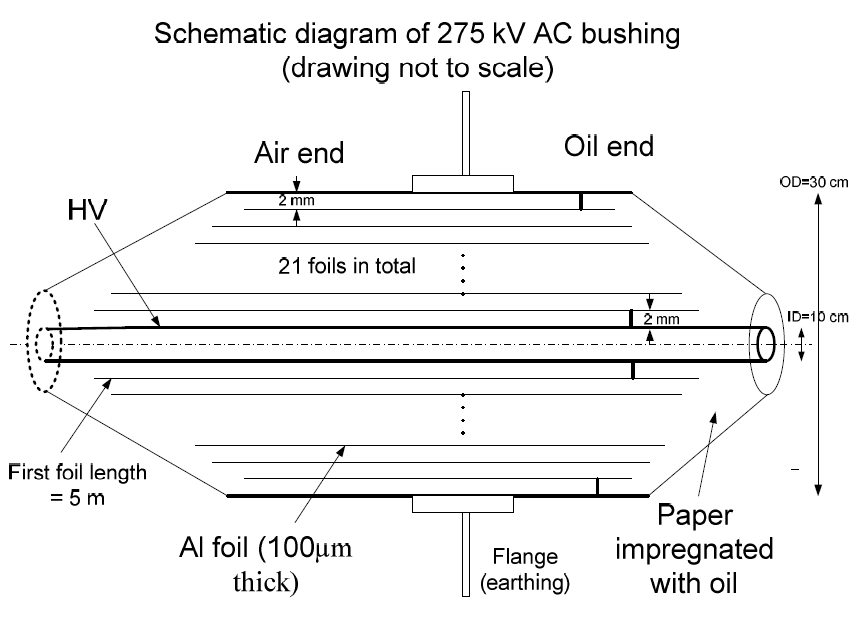
\includegraphics[width = 0.7\textwidth]{ReferenceDiagram.png}
   \caption{The reference problem taken from \cite{Chen14}}
   \label{figure:refproblem}
\end{figure}

\subsection{Design Issues} \label{Section:Design Issues}
In section \ref{ss:CapacitiveGrading} the initial information required for both radial and axial grading includes the length and radial displacement of the innermost foil.
In the reference design the following initial information is given.

\begin{table}[!htb]
\caption{Initial Information for Reference Design}
\label{table:initinfo}
\begin{center}
\begin{tabular}{cc}
\toprule
\textbf{Initial Information} & \textbf{Value} \\ \toprule
Conductor Diameter (ID) & $100mm$ \\
First Foil Length $L_1$ & $5000mm$ \\
First Foil Radius $r_1$&$52mm$ \\
Outer Bushing Diameter (OD) & $300mm$\\
Outer Foil Radius $r_21$ & $148mm$\\
\bottomrule
\end{tabular}
\end{center}
\end{table} 

This information intuitively fits radial grading best, since there is no requirement to assume the length of the outermost foil.
However, there is a discrepancy between the standard literature problem and the reference design.
The first foil is connected to the high voltage conductor, and the last foil is connected to the earthed flange.
This is to eliminate the electric field on the boundary interface as far as possible on both sides of the bushing, so that the voltage drop occurs exclusively inside the bushing insulation.

This has an impact on the calculations described in section \ref{ss:CapacitiveGrading}.
Since the innermost foil is at the same voltage as the conductor, there is no capacitance between them, as shown in figure \ref{figure:required assumptions}, hence the first foil shown on the diagram is not index 0 for the iterative calculation.
The derivation of the iterative equations assumes a capacitance between the current foil and the previous foil (or conductor) ($r_n,r_{n-1}$). 
The first foil in figure \ref{figure:refproblem} is therefore indexed as 0 and not 1.

\begin{figure}[!h]
   \centering
   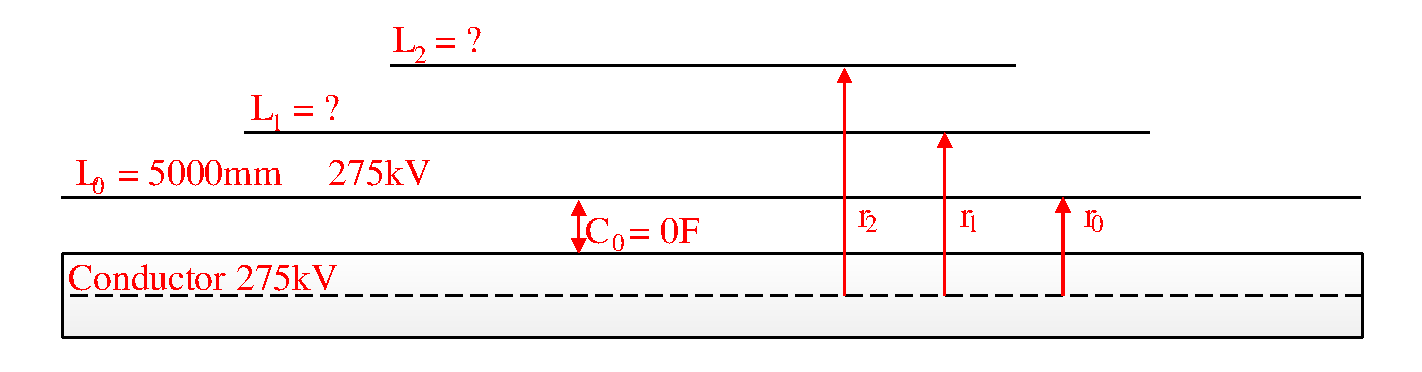
\includegraphics[width = \textwidth]{AssumptionExplanation.pdf}
   \caption{Diagram to explain the assumptions required}
   \label{figure:required assumptions}
\end{figure}

This means that there is not sufficient initial information to proceed with ether radial or axial grading, since the first non-connected foil length $L_1$ is not given.
The iterative equations require the first non-connected foil length $L_1$ for radial ( $L_1$ \& $r_1$ for axial) grading to be known as shown in equation \ref{eq:ref0forl1} and \ref{eq:ref0}. 
In axial grading all radii variables are known due to the even spacings under radial grading. In the axial grading case, the length of foils are known due to known parameters $b_{ln}$ and $b_{rn}$.

\begin{equation}
   \label{eq:ref0forl1}
   L_{2} = L_{1}\displaystyle\frac{{ln(\displaystyle\frac{r_{2}}{r_{1}})} }{ln(\displaystyle\frac{r_{1}}{r_{0}})} \qquad (Radial \; grading)
\end{equation}
\begin{equation}
  \label{eq:ref0}
  \displaystyle r_2= \displaystyle  r_{1} \displaystyle \exp\big( \displaystyle  \frac{L_2}{L_{1}}ln(\displaystyle \frac{r_1}{r_0})\big) \qquad (Axial \; grading)
\end{equation}



If this is not taken into account then a flawed design will be produced in both cases.
Equations \ref{eq:ref0wrongfilled} and \ref{eq:ref0wrongfilledA} show a wrongly described first iteration of the radial and axial grading formula. For radial grading the resulted design is shown in figure \ref{figure:flawedgraph}. This shows that the length of second foil is much bigger than the first foil. This is clearly wrong, and does not give the hyperbolic shape from the beginning of the foils.
\begin{equation}
   \label{eq:ref0wrongfilled}
   L_{1} = 5000\displaystyle\frac{{ln(\displaystyle\frac{56.8}{52})} }{ln(\displaystyle\frac{52}{50})}
   = 11256mm \qquad (Radial \; grading)
\end{equation}
\begin{equation}
\label{eq:ref0wrongfilledA}
   r_2 = 52 \displaystyle \exp\big( \frac{49418}{5000} \ln(\frac{52}{50})\big)= 54.05mm\Longrightarrow r_{21}=103.52mm \qquad (Axial \; grading)
\end{equation}

\begin{figure}[!h]
   \centering
   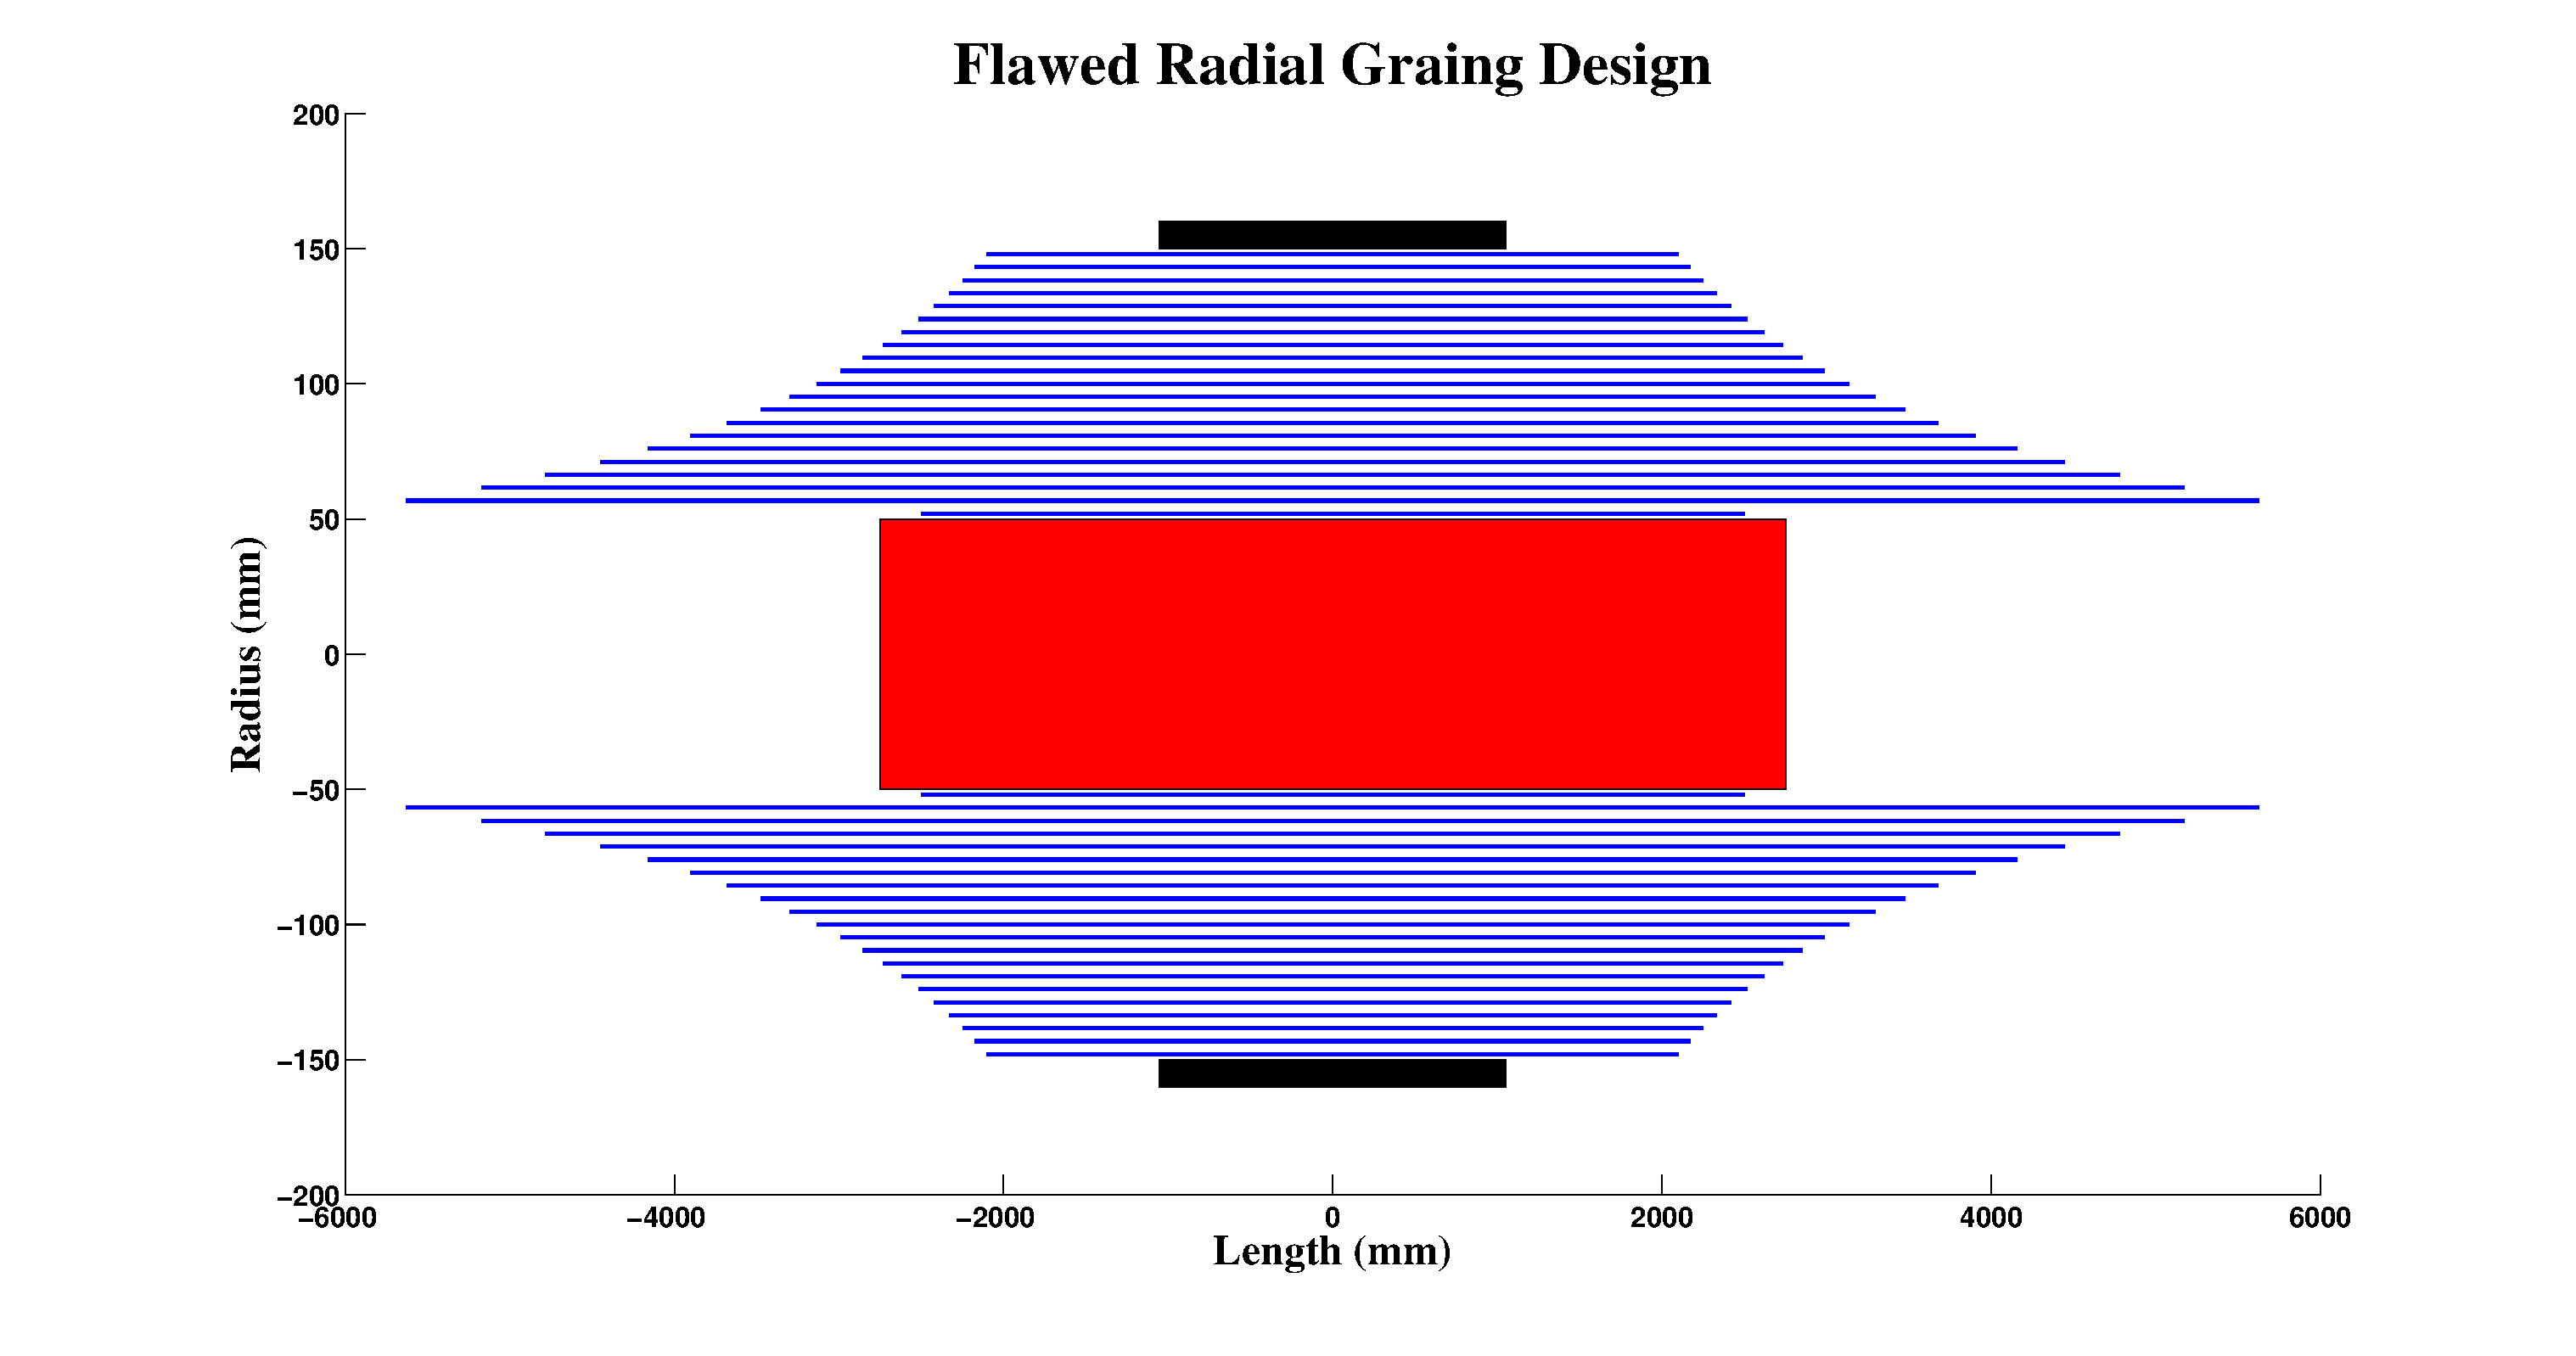
\includegraphics[width = 0.7\textwidth]{../Matlab_Calculations/Matlab_David/FlawedRadGradGraph.eps}
   \caption{Flawed Radial Grading Design}
   \label{figure:flawedgraph}
\end{figure}

In order to proceed with the calculations there must be an assumption of the length of the first unconnected foil.
A reasonable assumption is that this follows the hyperbolic shape of the other foils in radial grading and also in axial grading  it is assumed to be the first unconnected foil. These assumptions in both cases help to evenly distribute the electric field radially or axially accordingly.
To achieve this design mathematically, the following assumptions are made:
\begin{enumerate}
\item Foil $0$ is not connected to the HV conductor for both cases.
\item The conductor surface is spaced a distance of $S_n$ from foil $0$ in \textbf{radial grading}.
\item The conductor surface is spaced an adjustable distance from foil $0$ in \textbf{axial grading}.
\end{enumerate}
The reason of each assumption  according to the design constrains are explained as following:
\begin{itemize}[noitemsep,topsep=0pt]
\item Assumption 1 is required to be able to use the capacitor derived iterative formula on foil 0.
\item Assumption 2 is required so that the radial spacing is kept constant. 
\item Assumption 3 is required so that axial grading could be calculated with a varying parameter value for $r_0$. This makes it possible to adjust the initial gap so that the last foil will be placed exactly at 148mm. 

\end{itemize}
The first iteration has been calculated under these assumptions, giving the result in equations \ref{eq:ref0correct} and \ref{eq:ref0correct2} which are expected values.
The remainder of foil parameters can then be calculated using the iterative formulas in each grading.
\begin{equation}
   \label{eq:ref0correct}
   L_{1}
   = 5000\displaystyle\frac{{ln(\displaystyle\frac{56.8}{52})} }{ln(\displaystyle\frac{52}{47.2})}
   = 4558mm \qquad (Radial \; grading)
\end{equation}
\begin{equation}
\label{eq:ref0correct2}
   r_2 = 52 \exp\big( \frac{49418}{5000} \ln(\frac{52}{50-1.007})\big)= 55.15mm \Longrightarrow r_{21}\simeq 148mm \qquad (Axial \; grading)
\end{equation}


\section{Matlab Calculations}
Two Matlab scripts were developed for computation of radial and axial grading. 
These scripts were built to be easily customisable for any number of foils and any initial values, to cater for the calculation of improved designs. 
They also automatically outputs data in a form for direct input into the COMSOL model, auto-updates a \LaTeX  file containing the data to form results table and displays the results in both 2D and 3D plots for quick design verification.

\subsection{Matlab Radial Grading}
In case of radial grading  the code takes a required number of foils, and the inner and outer dimensions of the bushing, to calculate the radial location and length of each foil using the radial grading method as described in section \ref{ss:CapacitiveGrading} and also using the assumptions made for redial grading design on \ref{Section:Design Issues}. 


For current design with specified parameters, the script plots the calculated foil positions in a 3D graph shown in figure \ref{Figure:Both21plots}. Also the 2D plot of this design is shown in  figure \ref{Figure:21plot2}. This figure illustrates  the hyperbolic shape which was expected for radial grading.
These figures allows a quick verification of the scripts accuracy before proceeding to simulation.
%\begin{figure}[h!]
% \centering
%  \includegraphics[height = 6cm ]{../Matlab_Calculations/Matlab_David/Designeactualsize.eps} 
%  	\label{Figure:21plot1}
%  \caption{3D Representation of foil radial position and length}
%  \label{Figure:Both21plots}
%\end{figure}
%\begin{figure}[h!]
%  \centering
%   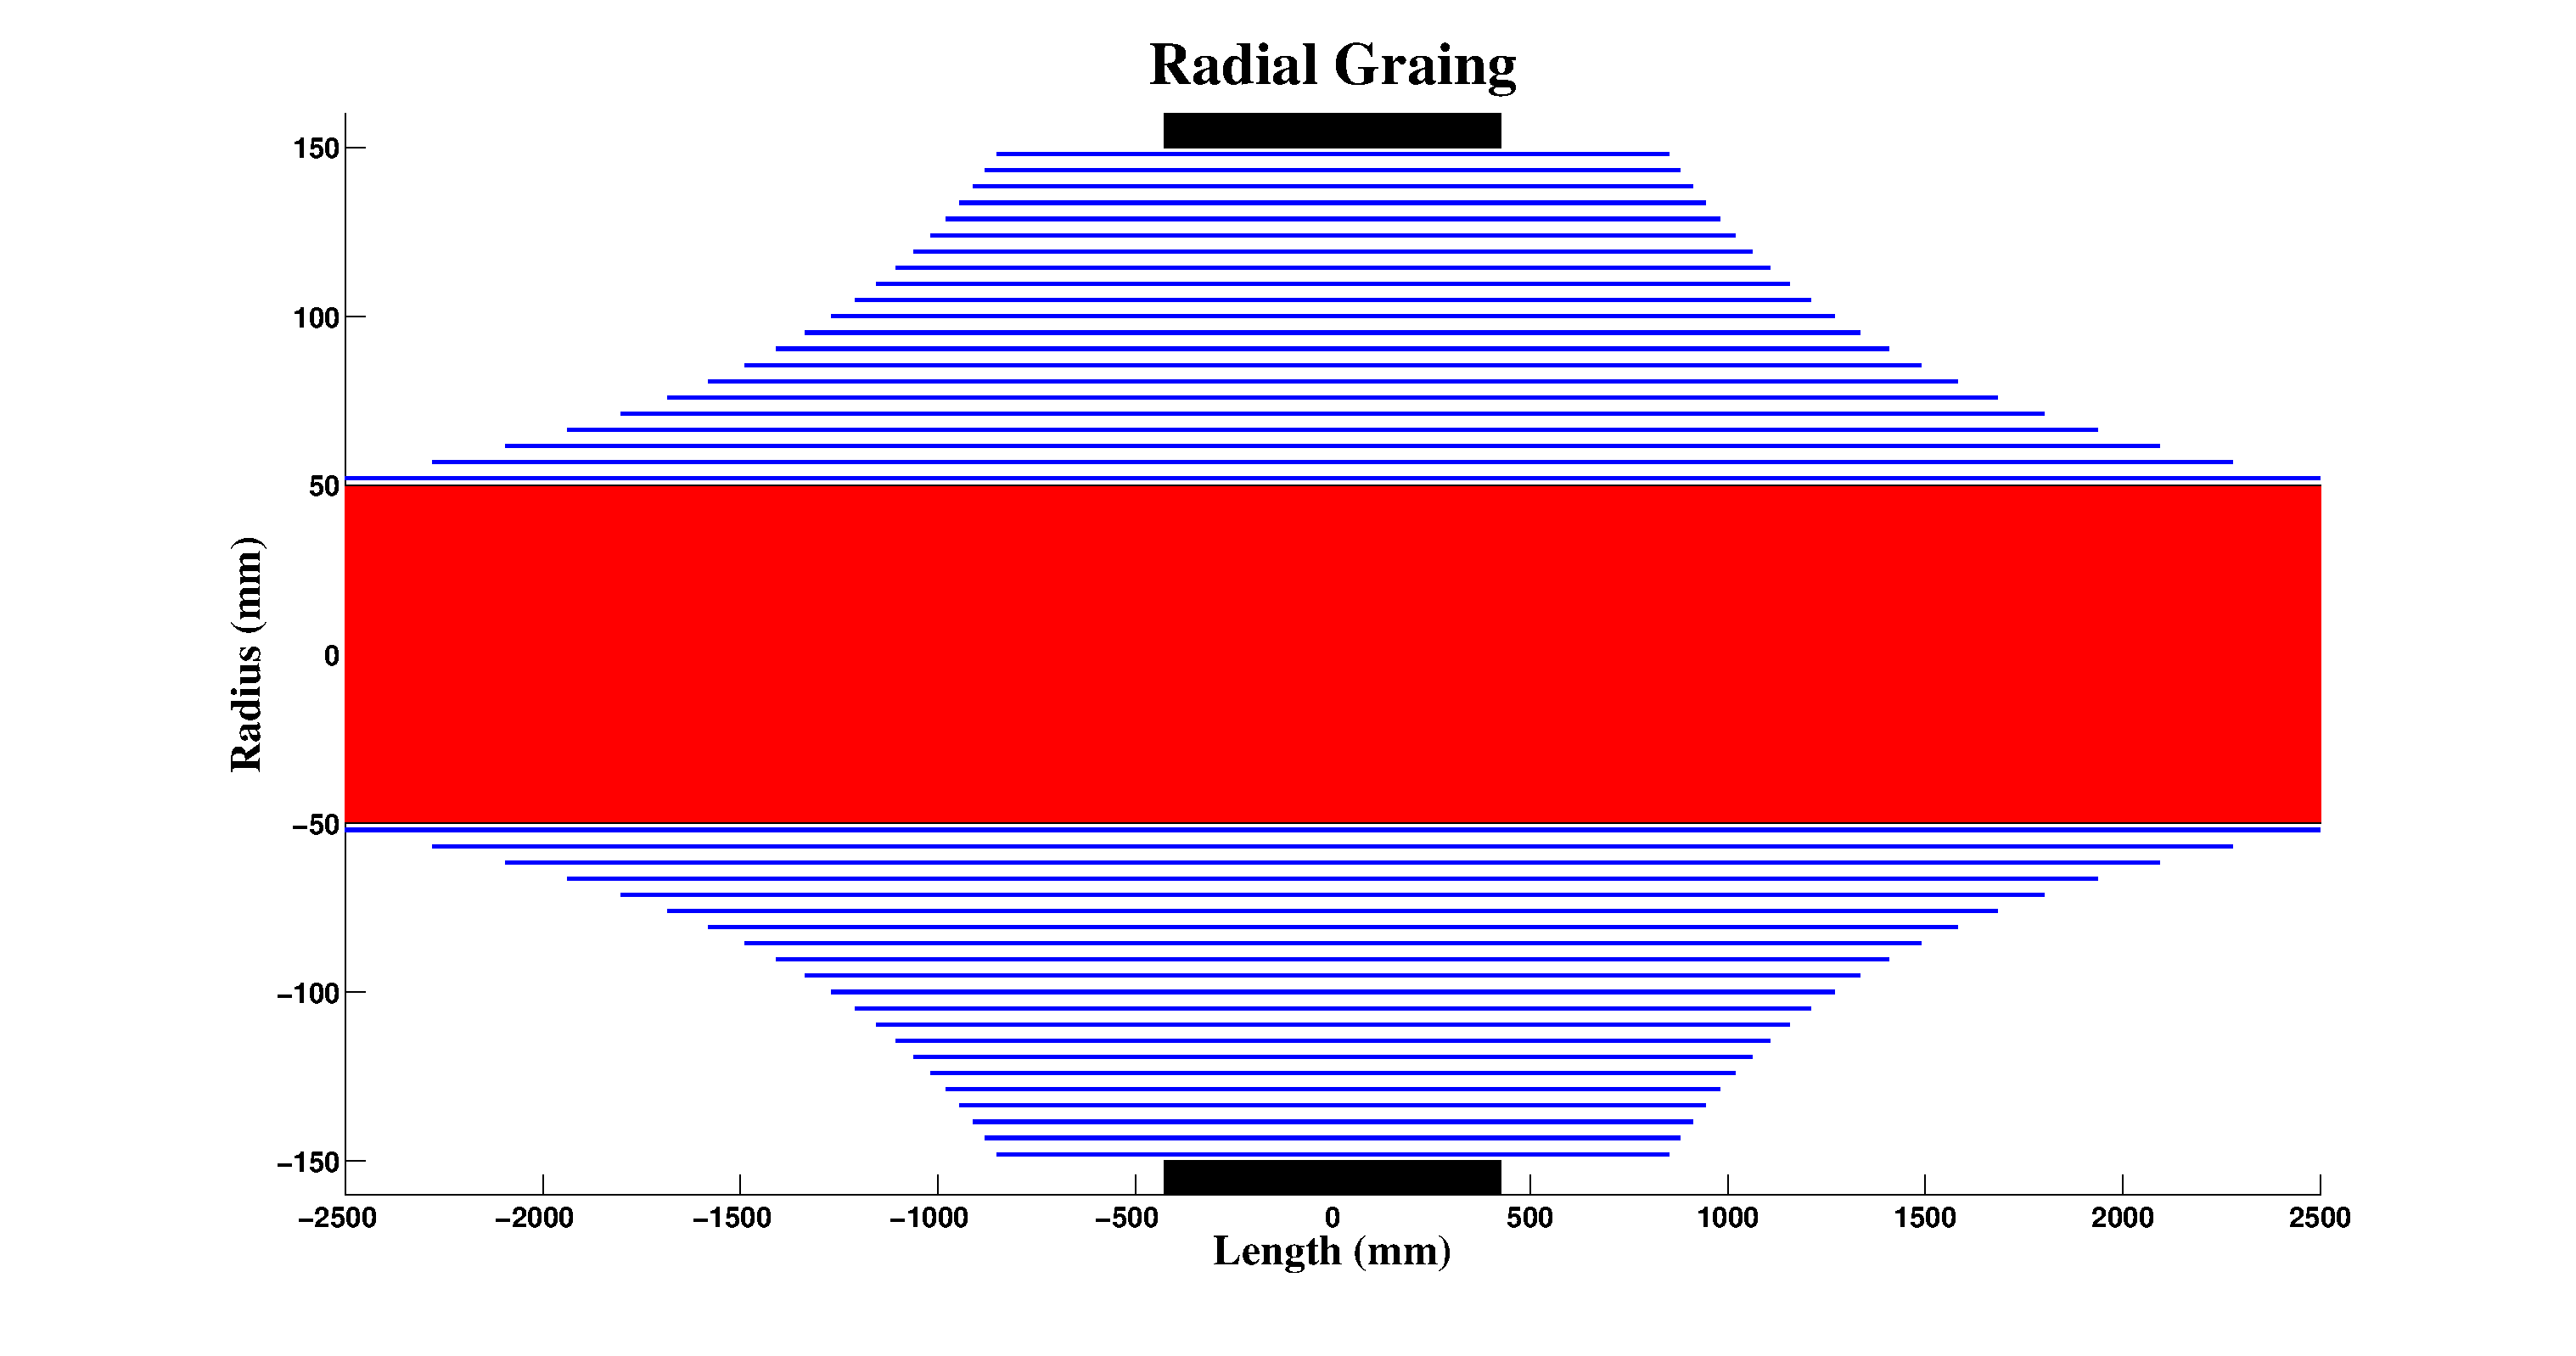
\includegraphics[height = 5cm]{../Matlab_Calculations/Matlab_David/2DRadial.eps} 
%   \caption{2D Representation of foil radial position and length}
%  	\label{Figure:21plot2}    
%\end{figure}
\begin{figure}[h!]
\centering
\begin{subfigure}[3D Representation of foil radial position and length]{
\includegraphics[height = 4.1cm]{../Matlab_Calculations/Matlab_David/Designeactualsize.eps} 
  	\label{Figure:21plot1}}
\end{subfigure}
\begin{subfigure}[2D Representation of foil radial position and length]{
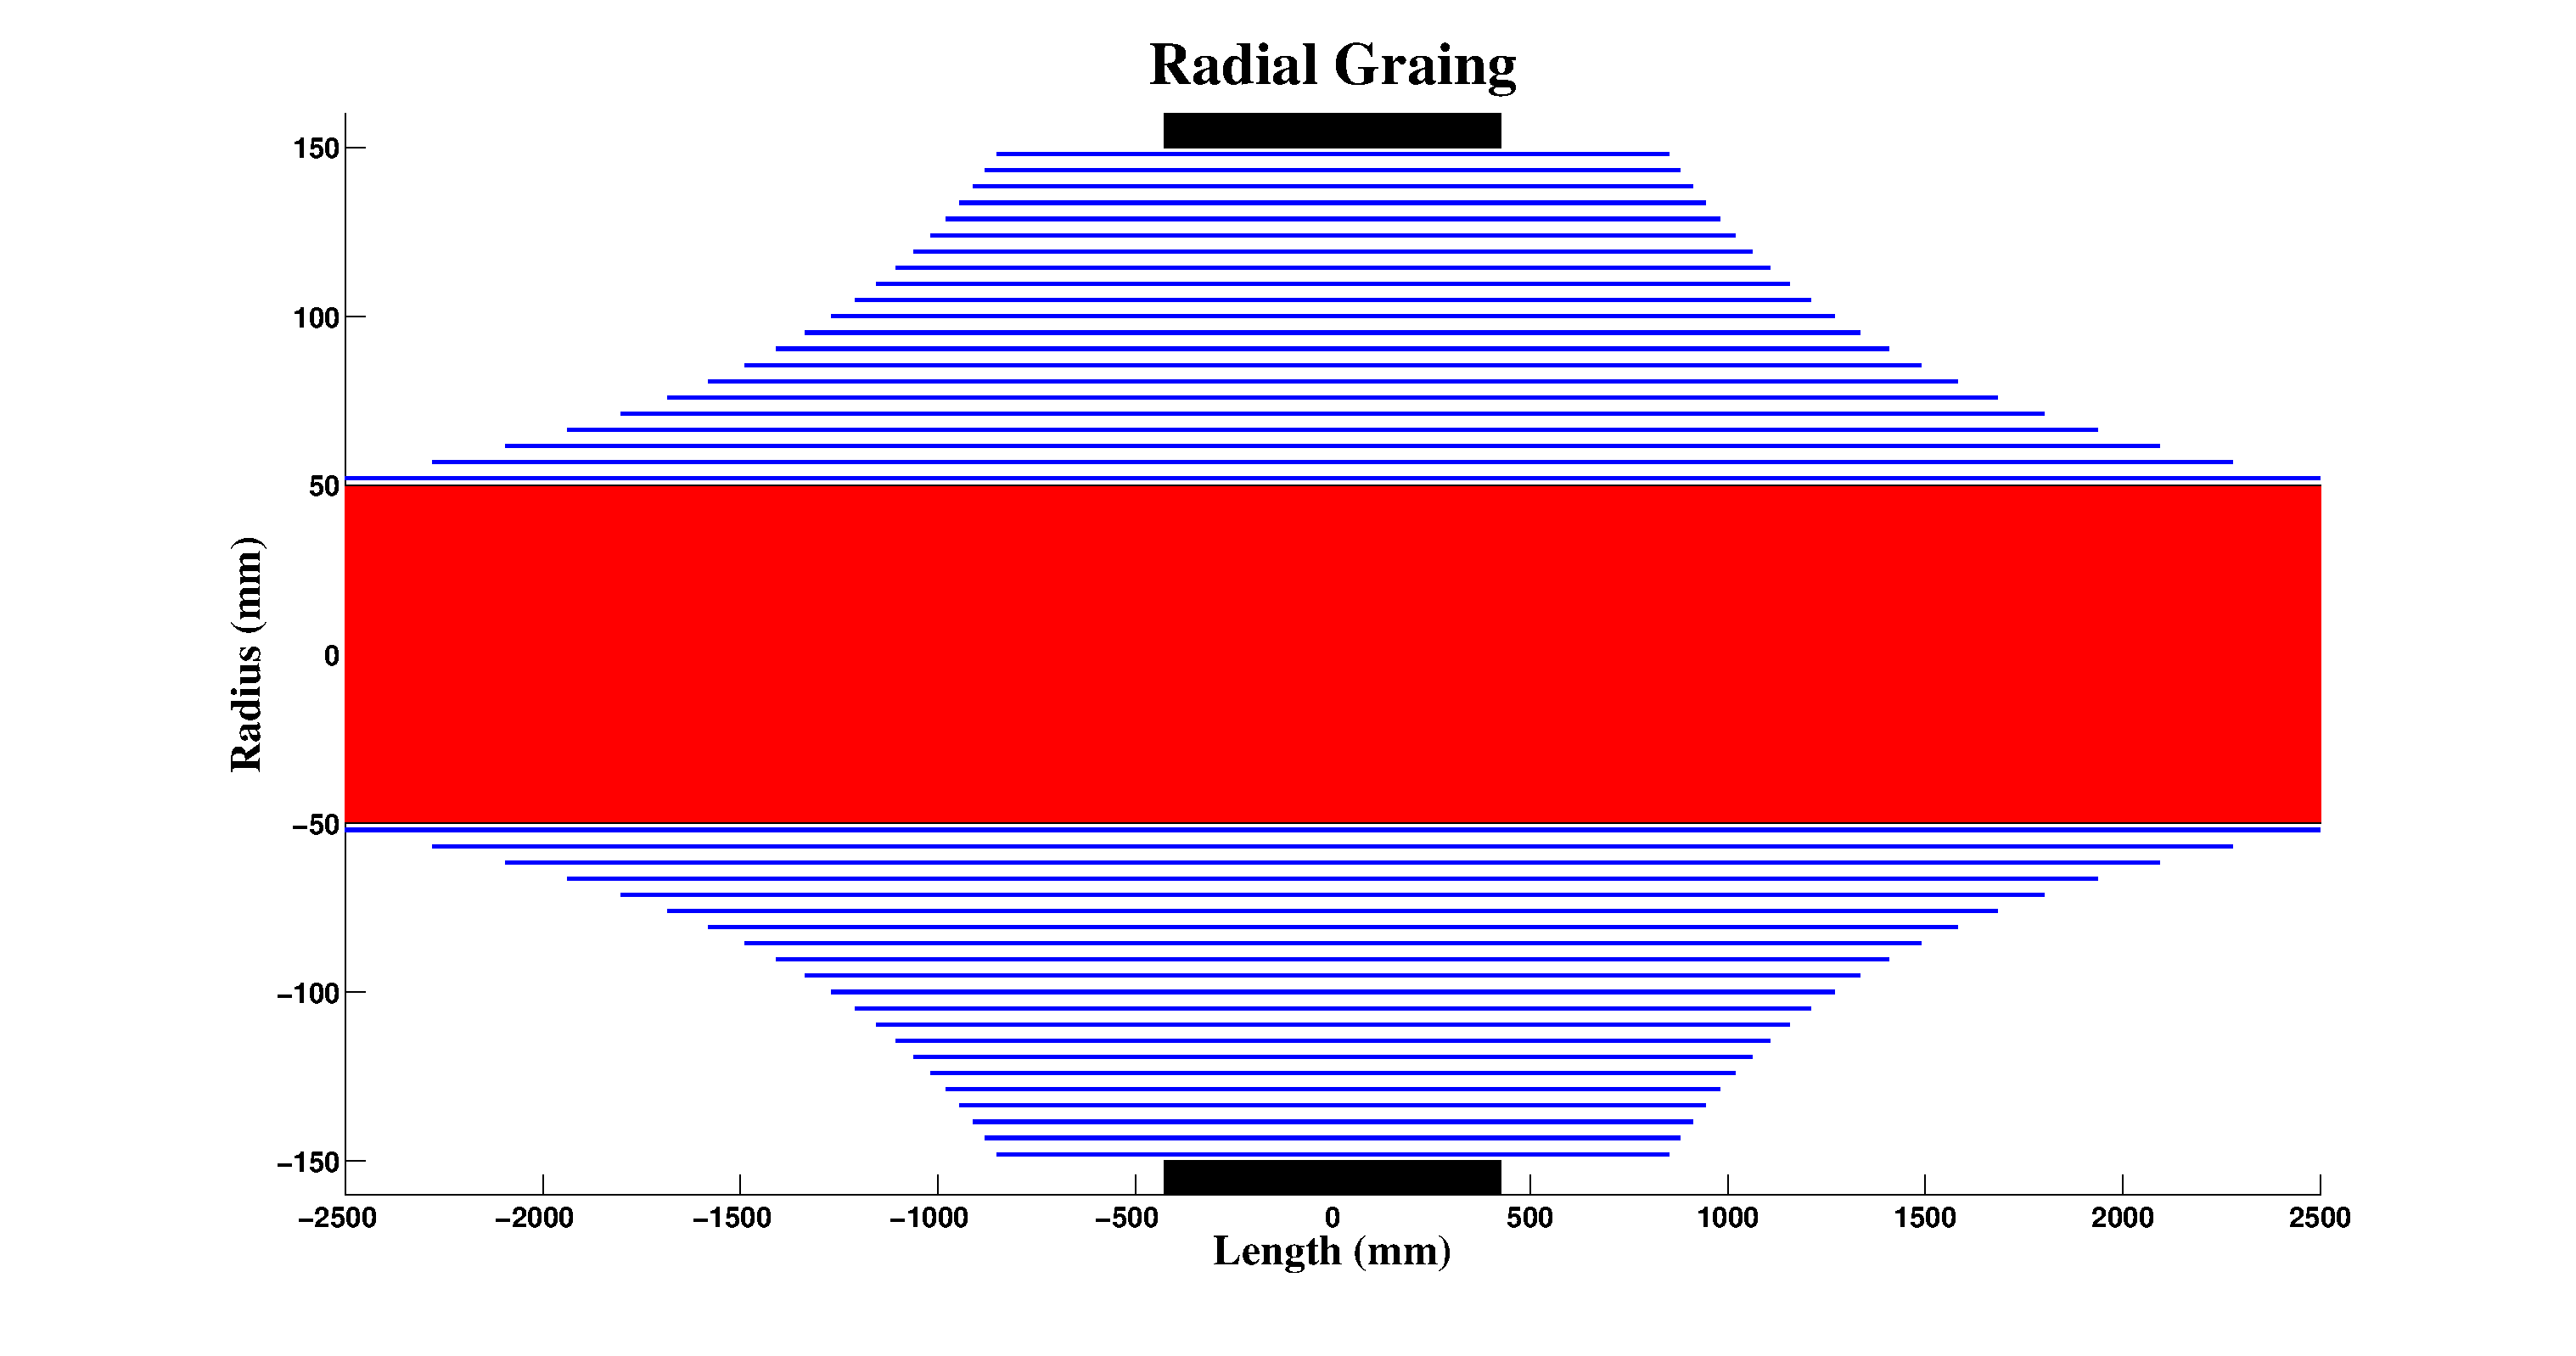
\includegraphics[height = 4.1cm]{../Matlab_Calculations/Matlab_David/2DRadial.eps}    
 	\label{Figure:21plot2}  }
\end{subfigure}
\caption{Matlab Generated Plots of Geometric Radial Design}
 \label{Figure:Both21plots}
\end{figure}





Table \ref{table:radialvals} shows the values obtained for radial grading.
The final information required to be able to proceed to the axial simulation phase is the relative permittivity of each material.
This was gathered from \cite{Ahmed11} and is shown in table \ref{table:perm}.

\begin{table}[!htb]
\caption{Radial Grading Calculations Results}
\label{table:radialvals}
\begin{center}
\begin{tabular}{cc}
\toprule
\textbf{Radius(mm)} & \textbf{Length(mm)} \\ \toprule
52.00 & 5000.00 \\
56.80 & 4558.22 \\
61.60 & 4188.21 \\
66.40 & 3873.79 \\
71.20 & 3603.30 \\
76.00 & 3368.13 \\
80.80 & 3161.78 \\
85.60 & 2979.27 \\
90.40 & 2816.68 \\
95.20 & 2670.92 \\
100.00 & 2539.51 \\
104.80 & 2420.43 \\
109.60 & 2312.01 \\
114.40 & 2212.90 \\
119.20 & 2121.93 \\
124.00 & 2038.15 \\
128.80 & 1960.73 \\
133.60 & 1888.98 \\
138.40 & 1822.29 \\
143.20 & 1760.16 \\
148.00 & 1702.12 \\
150.00 & 851.06 \\
\bottomrule
\end{tabular}
\end{center}
\end{table}


\begin{table}[!htb]
\begin{center}
\begin{tabular}{cc}
\toprule
\textbf{Material} & \textbf{Relative Permittivity ($\epsilon_r$)} \\ \toprule
Air & $1$ \\
Oil &$ 2.2$ \\
Paper Impregnated with Oil &$ 4$ \\
Aluminium & $10^8$\\
\bottomrule
\end{tabular}
\end{center}
\caption{Relative Permittivity of Materials}
\label{table:perm}
\end{table}

\subsection{Matlab Axial Grading}
The axial grading script is similar to the radial grading script in design. 
However, as it is explain in reference \cite{David1}, the constant difference of foil length in oil and air side of bushing ($b_{air}$, $b_{oil}$) is calculated by considering the value of flash over distance $L_{air}$ and $L_{oil}$. 
These values are calculated by using the fact that average electric field strength along the boundary surface in oil side should be 3 to 4 Kv/cm and nearly 9 to 12 Kv/cm  in air side of the bushing. 
These values are calculated using equation \ref{eq:bes}. 
 
\begin{equation}
\label{eq:bes}
 b_{air} = \displaystyle \frac{  \Delta V}{900 \;^v/_{mm}} \qquad \qquad
 b_{oil} = \displaystyle \frac{  \Delta V}{300 \;^v/_{mm}}
\end{equation}

Additionally, as shown in equation \ref{eq:ref02}, in the calculation of $r_2$ a parameter called $R_{parameter}$ is subtracted form $r_0$  to change the position of assumed conductor surface. 
The radius of the last foil ($r_{21}$) could be correctly adjusted by making changes in this parameter and executing the script. $R_{parameter}=1.007mm$ was the best value found for this design.
\begin{equation}
  \label{eq:ref02}
  \displaystyle r_2= \displaystyle  r_{1} \displaystyle \exp\big( \displaystyle  \frac{L_2}{L_{1}}ln(\displaystyle \frac{r_1}{r_0-R_{parameter}})\big) 
\end{equation}

The script plots 2D and 3D plots of axial grading to the user. Figure \ref{Figure:21plot221} illustrates the 3D configuration of design's axial bushing.  
The 2D plot of this design, which is shown in figure \ref{Figure:21plot22}, shows linear reduction on foil length on both sides. 
It also illustrates that $b_{air}>b_{oil} $ as it was expected due to the relative permittivity of each material.  
Finally the calculated values for axial grading, using this design method, are shown in \ref{table:axialvals}. 
These values along the given parameters in table \ref{table:perm} were used for COMSOL simulations of this axial grading design.
%\begin{figure}[h!]
%  \centering
%   \includegraphics[height = 8cm]{../Matlab_Calculations/Matlab_David/Axial3D.eps} 
%   \caption{2D Representation of foil radial position and length}
%  	\label{Figure:21plot221}    
%\end{figure}
%\begin{figure}[h!]
%  \centering
%   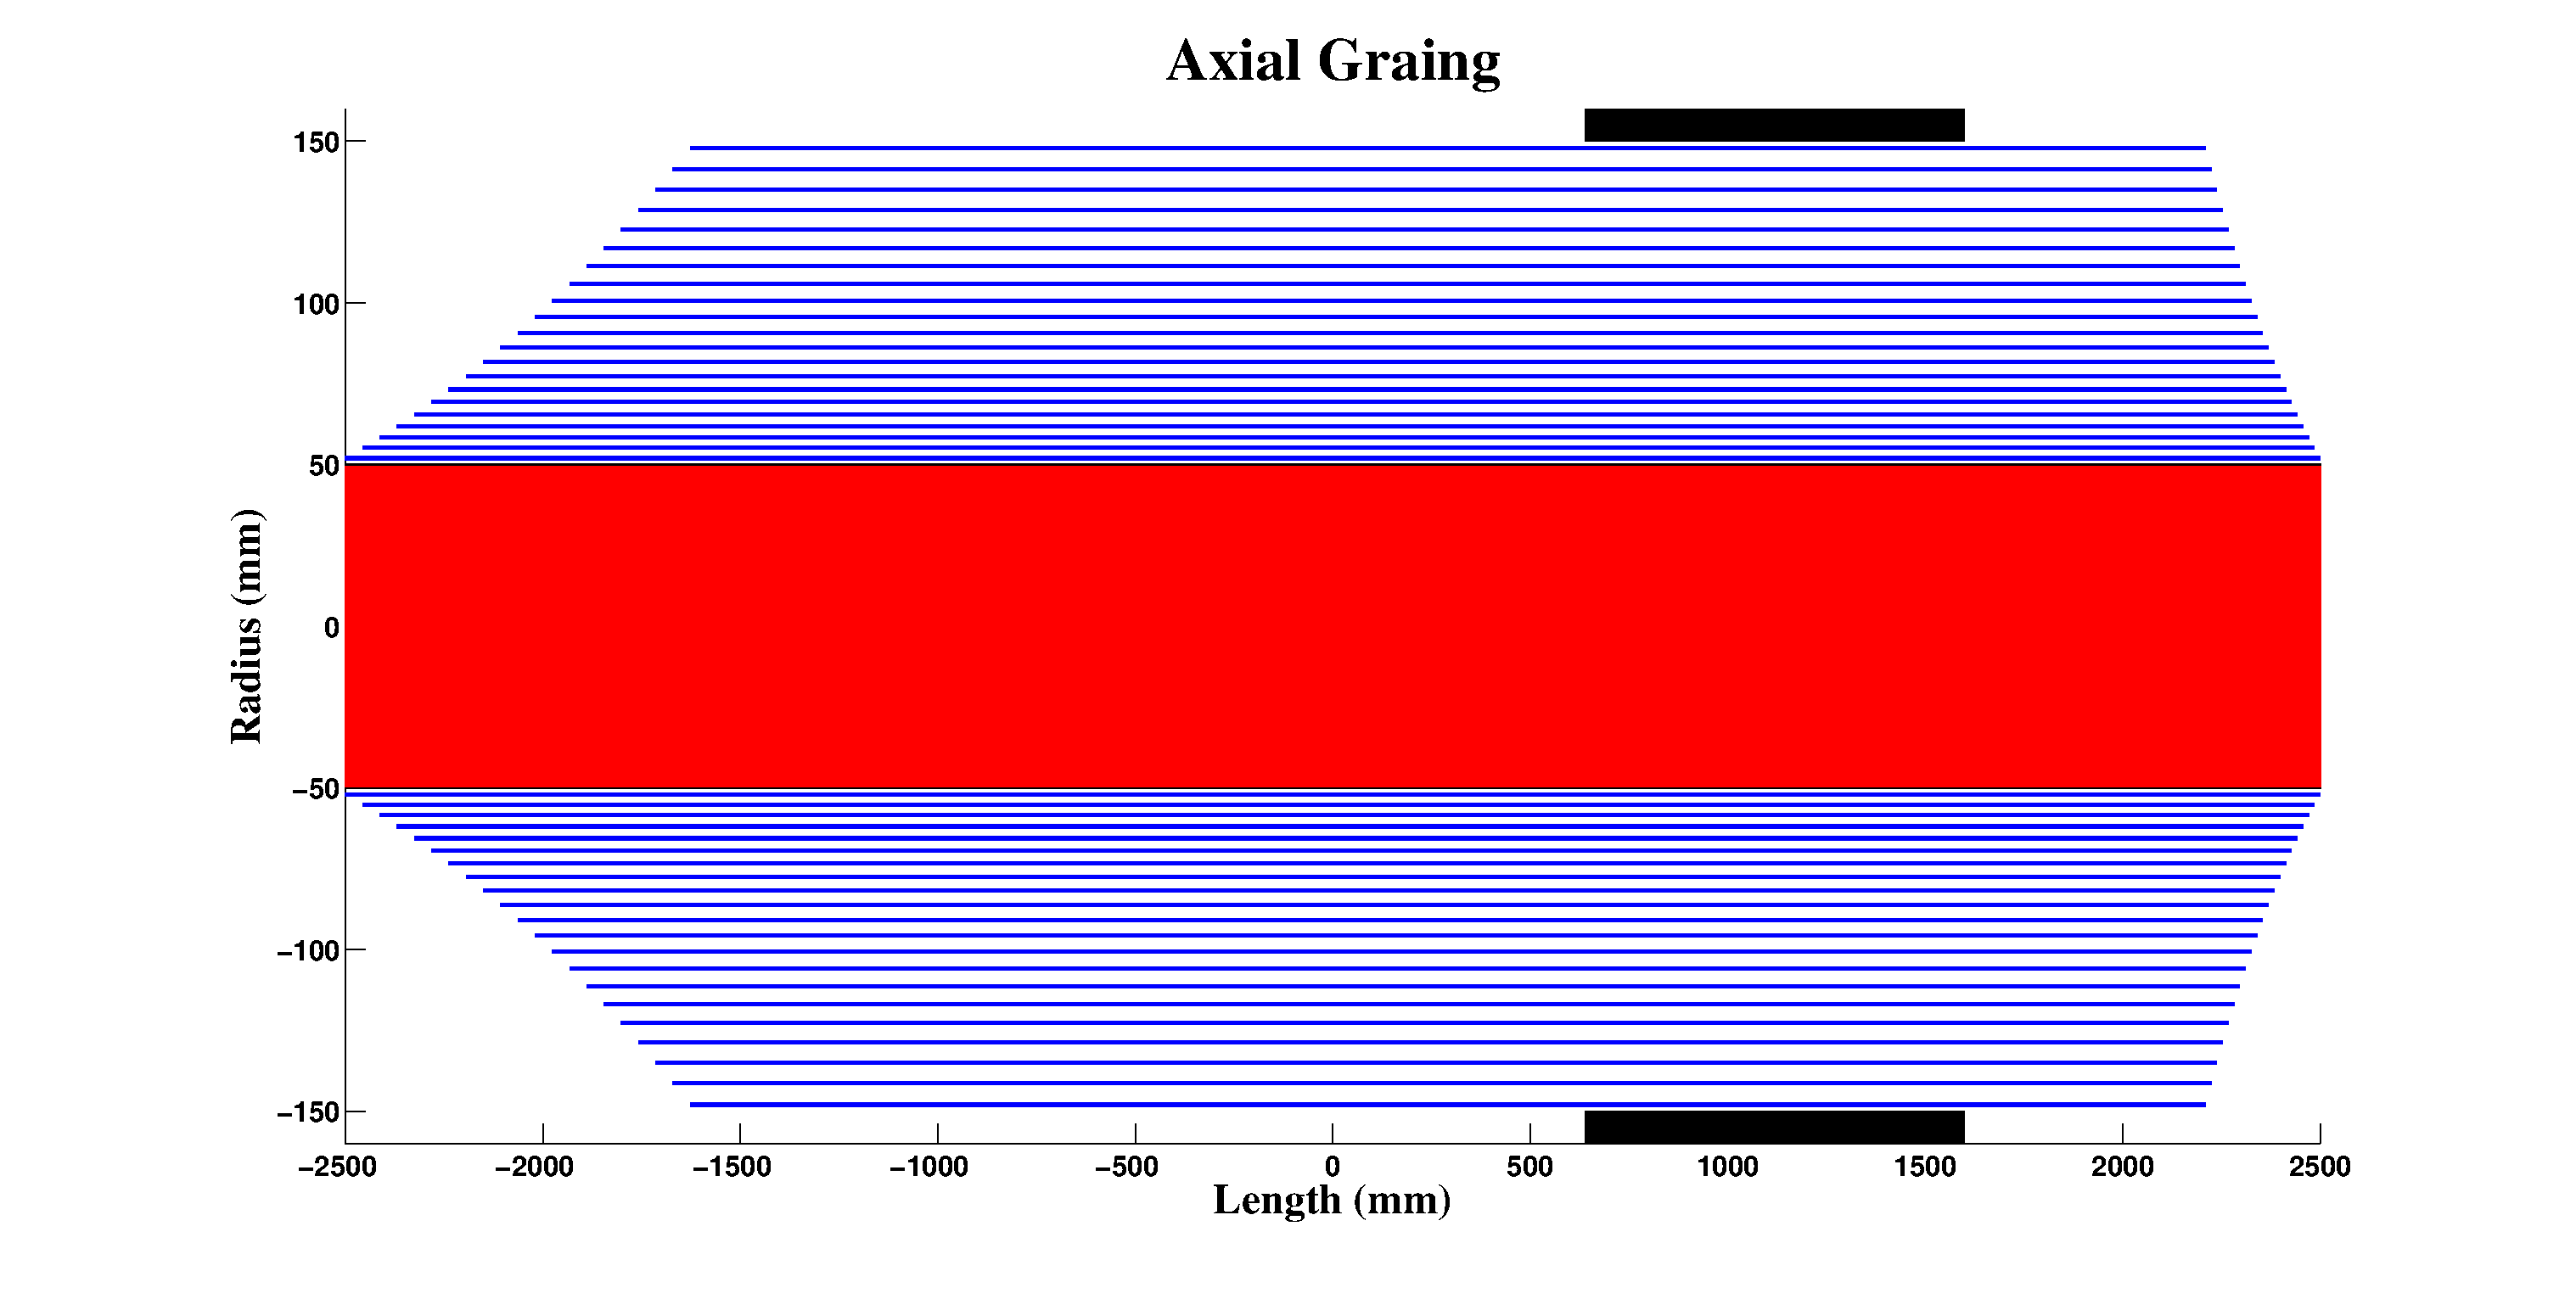
\includegraphics[height = 5cm]{../Matlab_Calculations/Matlab_David/Axsial2D.eps} 
%   \caption{2D Representation of foil radial position and length}
%  	\label{Figure:21plot22}    
%\end{figure}
%\begin{table}[!htb]
\caption{Axial Grading Calculations Results}
\label{table:axiallvals}
\begin{center}
\begin{tabular}{cc}
\toprule
\textbf{Radius(mm)} & \textbf{Length(mm)} \\ \toprule
52.00 & 5000.00 \\
55.15 & 4941.80 \\
58.46 & 4883.61 \\
61.92 & 4825.41 \\
65.53 & 4767.21 \\
69.32 & 4709.02 \\
73.26 & 4650.82 \\
77.39 & 4592.62 \\
81.68 & 4534.43 \\
86.15 & 4476.23 \\
90.81 & 4418.03 \\
95.65 & 4359.84 \\
100.68 & 4301.64 \\
105.90 & 4243.44 \\
111.32 & 4185.25 \\
116.93 & 4127.05 \\
122.73 & 4068.85 \\
128.74 & 4010.66 \\
134.95 & 3952.46 \\
141.35 & 3894.26 \\
147.96 & 3836.07 \\
149.96 & 1918.03 \\
\bottomrule
\end{tabular}
\end{center}
\end{table}


\begin{figure}[h!]
\centering
\begin{subfigure}[3D Representation of foil radial position and length]{
\includegraphics[height = 3.9cm]{../Matlab_Calculations/Matlab_David/Axial3D.eps} 
  	\label{Figure:21plot221}}
\end{subfigure}
\begin{subfigure}[2D Representation of foil radial position and length]{
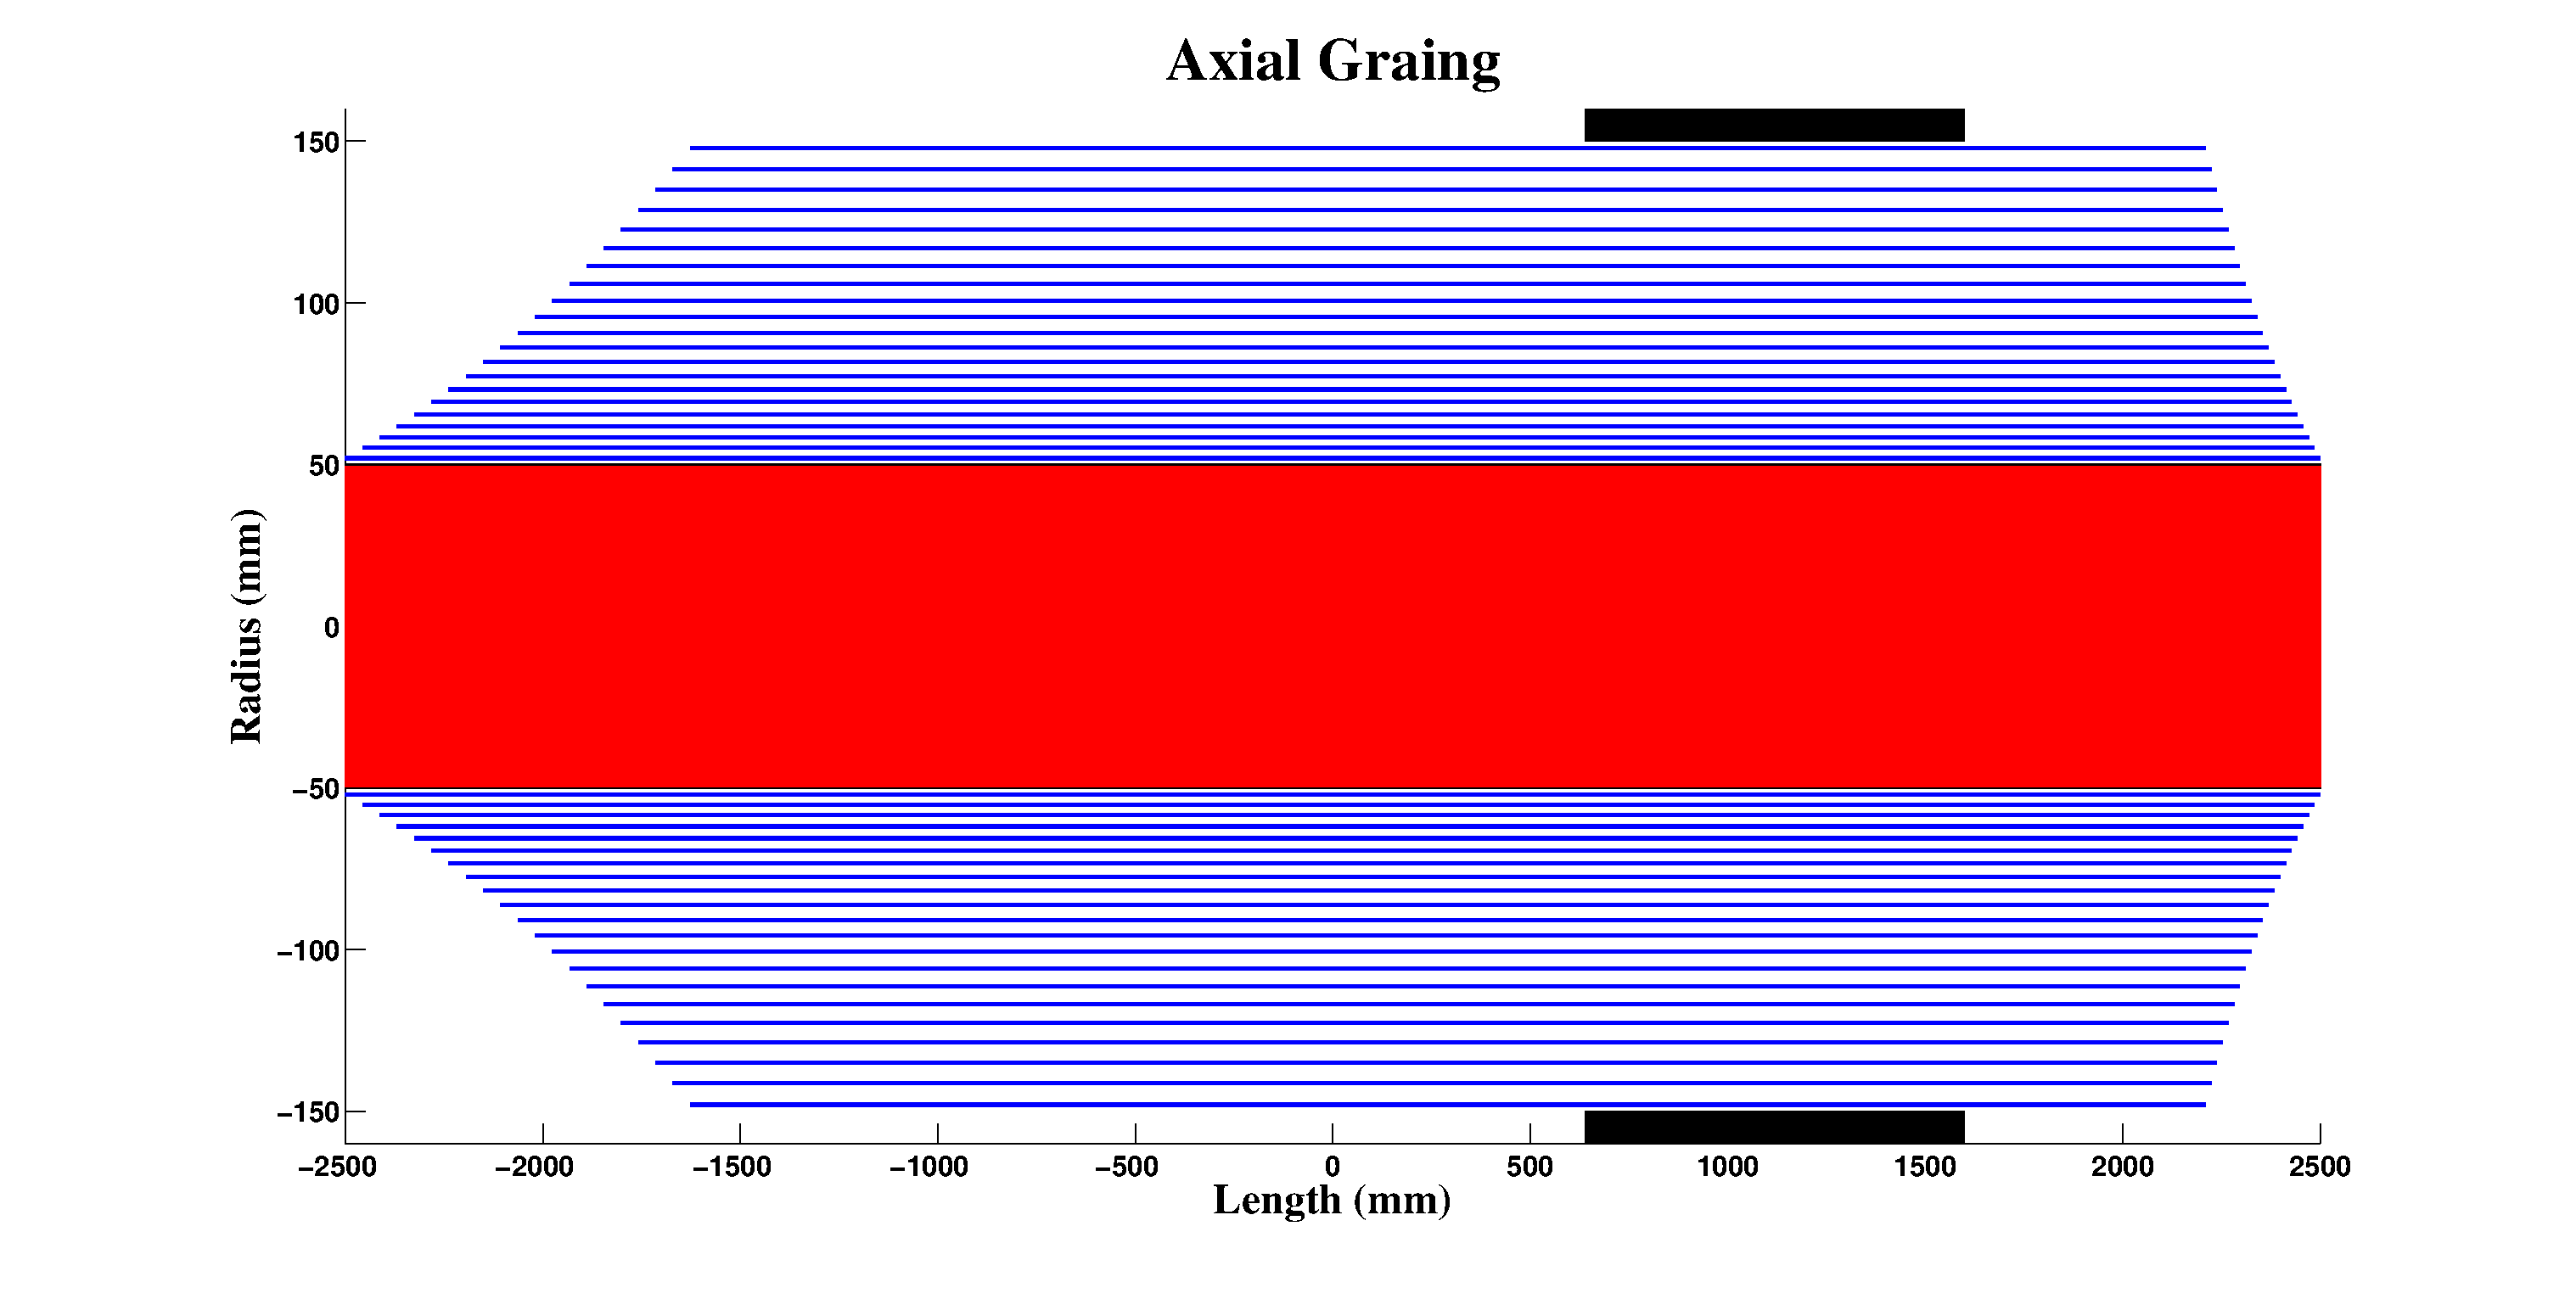
\includegraphics[height = 3.9cm]{../Matlab_Calculations/Matlab_David/Axsial2D.eps}    
 	\label{Figure:21plot22}  }
\end{subfigure}
\caption{Matlab Generated Plots of Geometric Axial Design}
 \label{Figure:Both22plots}
\end{figure}

\begin{table}[!htb]
\caption{Axial Grading Calculations Results}
\label{table:axiallvals}
\begin{center}
\begin{tabular}{cc}
\toprule
\textbf{Radius(mm)} & \textbf{Length(mm)} \\ \toprule
52.00 & 5000.00 \\
55.15 & 4941.80 \\
58.46 & 4883.61 \\
61.92 & 4825.41 \\
65.53 & 4767.21 \\
69.32 & 4709.02 \\
73.26 & 4650.82 \\
77.39 & 4592.62 \\
81.68 & 4534.43 \\
86.15 & 4476.23 \\
90.81 & 4418.03 \\
95.65 & 4359.84 \\
100.68 & 4301.64 \\
105.90 & 4243.44 \\
111.32 & 4185.25 \\
116.93 & 4127.05 \\
122.73 & 4068.85 \\
128.74 & 4010.66 \\
134.95 & 3952.46 \\
141.35 & 3894.26 \\
147.96 & 3836.07 \\
149.96 & 1918.03 \\
\bottomrule
\end{tabular}
\end{center}
\end{table}
